\paragraph{GET /:lang/user/training/question} % richiesta che ritorna la prossima domanda dell'allenamento
\begin{itemize}
\item \textbf{Successo}\\
Questo scenario rappresenta una richiesta che ritorna la prossima domanda nella modalità Allenamento.

\begin{figure}[ht]
	\centering
	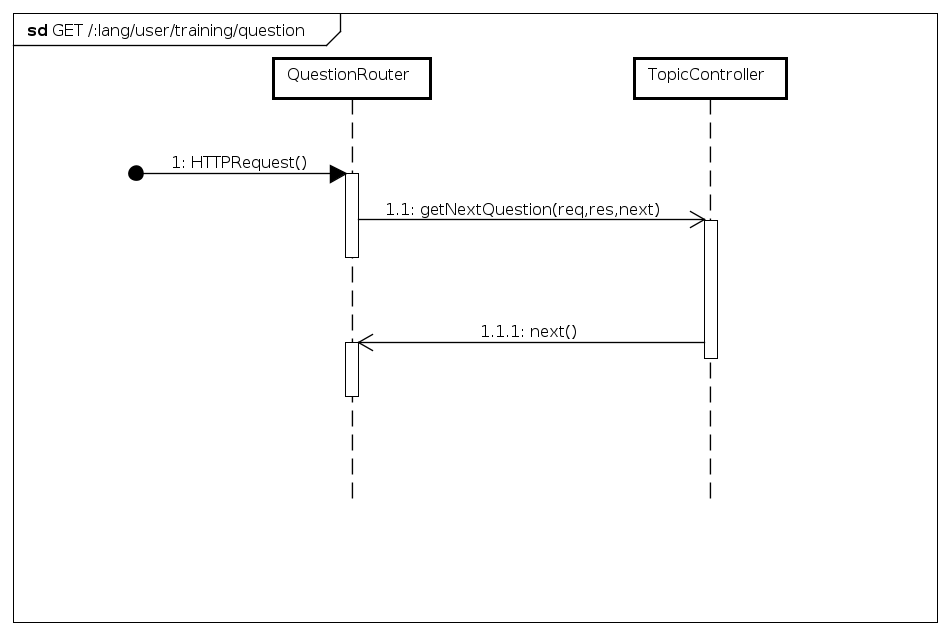
\includegraphics[scale=0.45]{UML/DiagrammiDiSequenza/Back-end/GET__lang_user_training_question_success.png}
	\caption{Successo: GET /:lang/user/training/question}
\end{figure}
\FloatBarrier

\item \textbf{Fallimento}\\
Questo scenario rappresenta una richiesta che ritorna la prossima domanda nella modalità Allenamento non andata a buon fine; in questo caso il modulo \texttt{TopicController} ritornerà un \texttt{next(err)} al router che avrà il compito di reinstradarlo (indirizzandolo verso \texttt{ErrorHandler}).

\begin{figure}[ht]
	\centering
	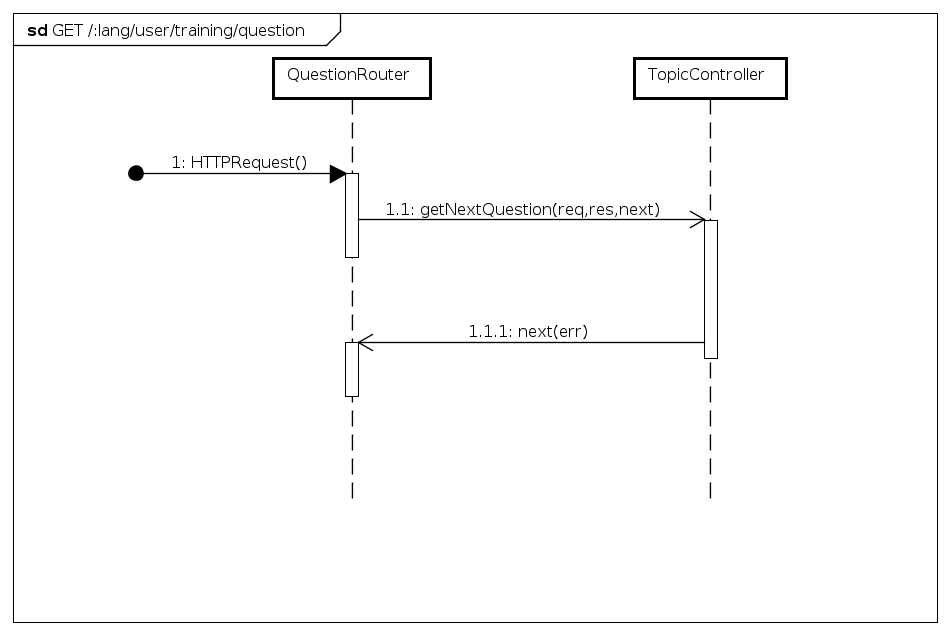
\includegraphics[scale=0.45]{UML/DiagrammiDiSequenza/Back-end/GET__lang_user_training_question_failure.png}
	\caption{Fallimento: GET /:lang/user/training/question}
\end{figure}
\FloatBarrier

\end{itemize}






\paragraph{PUT /:lang/user/:userId/training/userstatistics} % richiesta che aggiorna le statistiche dell'utente
\begin{itemize}
\item \textbf{Successo}\\
Questo scenario rappresenta una richiesta che aggiorna le statistiche di un utente dopo che ha risposto ad una domanda.

\begin{figure}[ht]
	\centering
	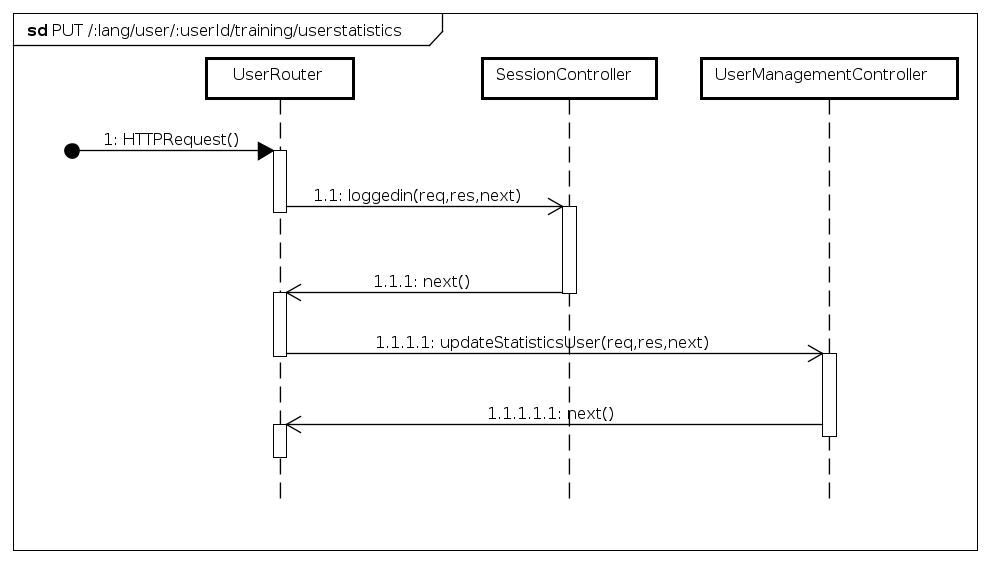
\includegraphics[scale=0.45]{UML/DiagrammiDiSequenza/Back-end/PUT__lang_user__userId_training_userstatistics_success.png}
	\caption{Successo: PUT /:lang/user/:userId/training/userstatistics}
\end{figure}
\FloatBarrier

\item \textbf{Fallimento}\\
Questo scenario rappresenta una richiesta che aggiorna le statistiche di un utente dopo che ha risposto ad una domanda non andata a buon fine; in questo caso il modulo \texttt{UserManagementController} ritornerà un \texttt{next(err)} al router che avrà il compito di reinstradarlo (indirizzandolo verso \texttt{ErrorHandler}).

\begin{figure}[ht]
	\centering
	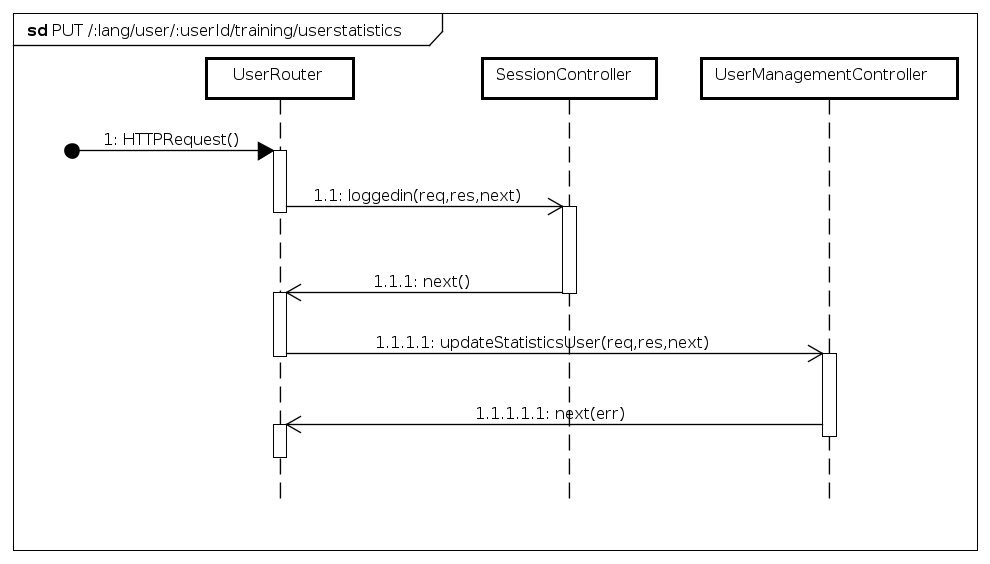
\includegraphics[scale=0.45]{UML/DiagrammiDiSequenza/Back-end/PUT__lang_user__userId_training_userstatistics_failure.png}
	\caption{Fallimento: PUT /:lang/user/:userId/training/userstatistics}
\end{figure}
\FloatBarrier

\end{itemize}








\paragraph{PUT /:lang/user/:userId/training/questionstatistics} % richiesta che aggiorna le statistiche della domanda
\begin{itemize}
\item \textbf{Successo}\\
Questo scenario rappresenta una richiesta che aggiorna le statistiche di una domanda a cui è stata data una risposta.

\begin{figure}[ht]
	\centering
	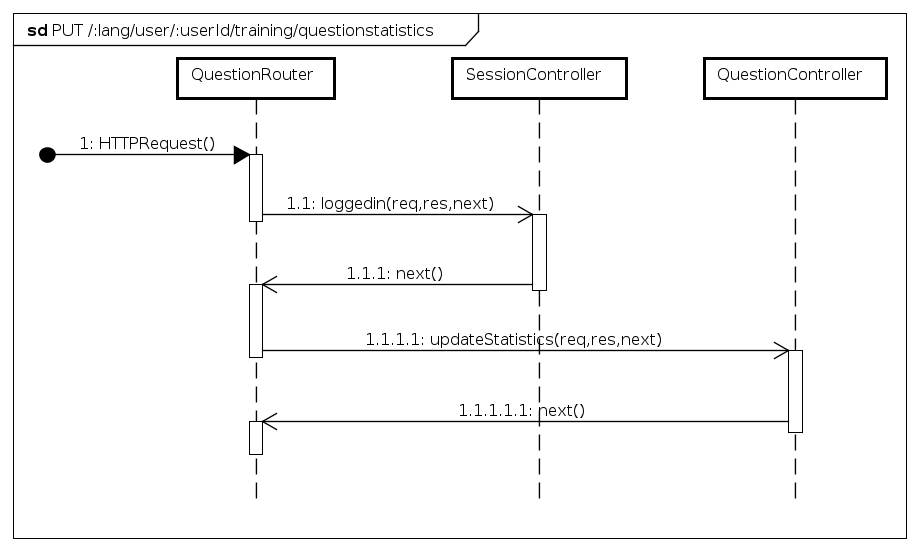
\includegraphics[scale=0.45]{UML/DiagrammiDiSequenza/Back-end/PUT__lang_user__userId_training_questionstatistics_success.png}
	\caption{Successo: PUT /:lang/user/:userId/training/questionstatistics}
\end{figure}
\FloatBarrier

\item \textbf{Fallimento}\\
Questo scenario rappresenta una richiesta che aggiorna le statistiche di una domanda a cui è appena stata data una risposta non andata a buon fine; in questo caso il modulo \texttt{QuestionController} ritornerà un \texttt{next(err)} al router che avrà il compito di reinstradarlo (indirizzandolo verso \texttt{ErrorHandler}).

\begin{figure}[ht]
	\centering
	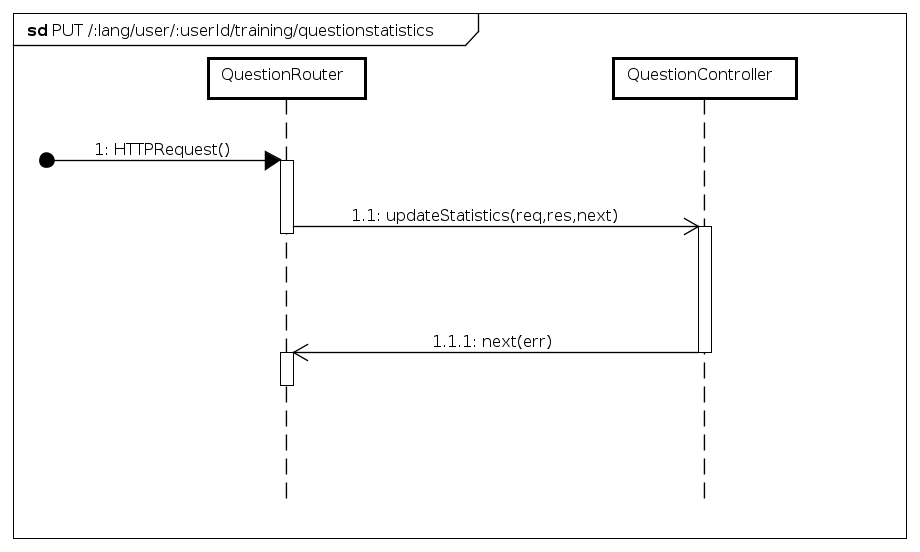
\includegraphics[scale=0.45]{UML/DiagrammiDiSequenza/Back-end/PUT__lang_user__userId_training_questionstatistics_failure.png}
	\caption{Fallimento: PUT /:lang/user/:userId/training/questionstatistics}
\end{figure}
\FloatBarrier

\end{itemize} 







\paragraph{PUT /:lang/user/training/userlevelupdate}
\begin{itemize}
\item \textbf{Successo}\\
Questo scenario rappresenta una richiesta che aggiorna il livello di un utente non autenticato per far sì che il sistema scelga domande adeguate alla sua preparazione.

\begin{figure}[ht]
	\centering
	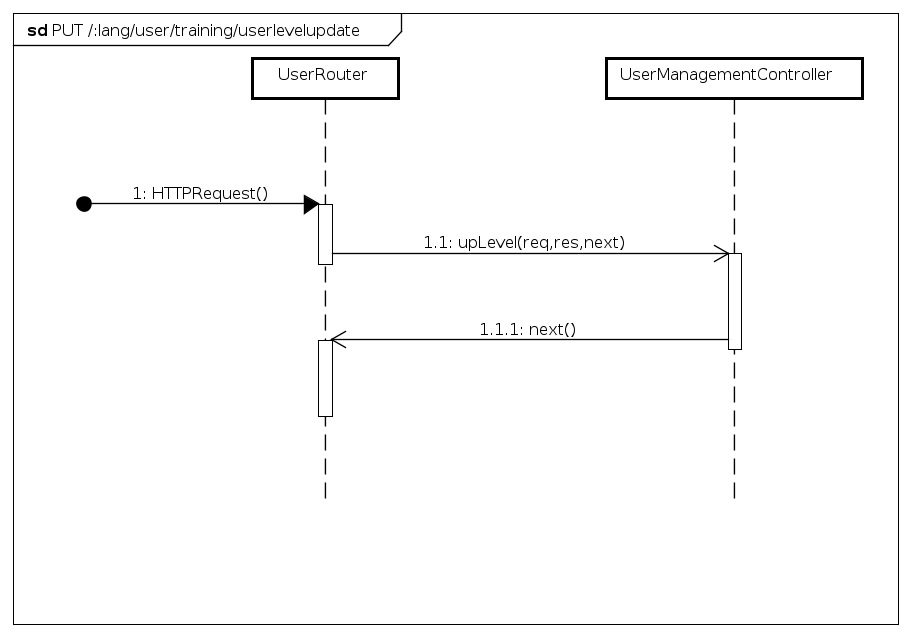
\includegraphics[scale=0.45]{UML/DiagrammiDiSequenza/Back-end/PUT__lang_user_training_userlevelupdate_success.png}
	\caption{Successo: PUT /:lang/user/training/userlevelupdate}
\end{figure}
\FloatBarrier

\item \textbf{Fallimento}\\
Questo scenario rappresenta una richiesta che aggiorna il livello di un utente non autenticato non andata a buon fine; in questo caso il modulo \texttt{UserManagementController} ritornerà un \texttt{next(err)} al router che avrà il compito di reinstradarlo (indirizzandolo verso \texttt{ErrorHandler}).

\begin{figure}[ht]
	\centering
	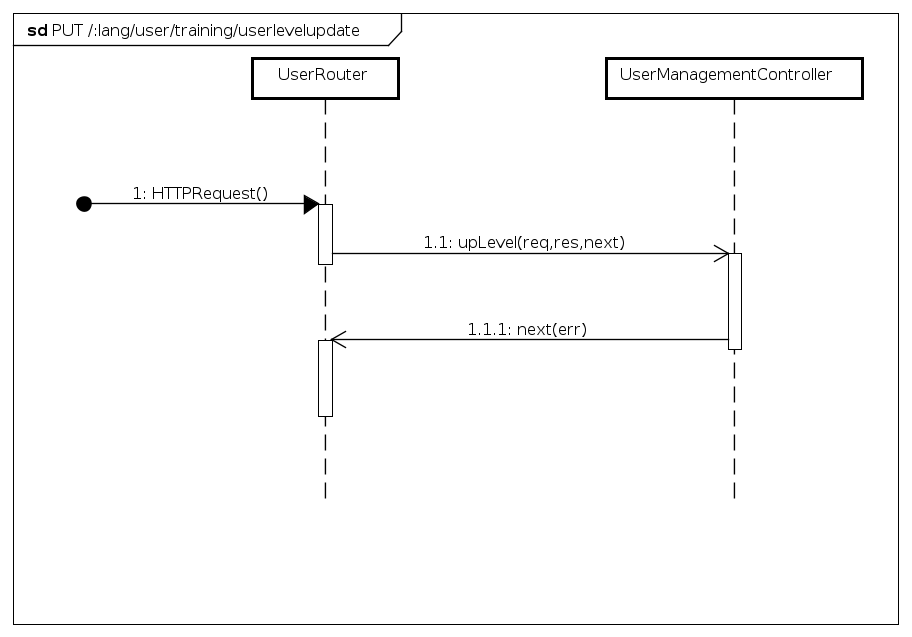
\includegraphics[scale=0.45]{UML/DiagrammiDiSequenza/Back-end/PUT__lang_user_training_userlevelupdate_failure.png}
	\caption{Fallimento: PUT /:lang/user/training/userlevelupdate}
\end{figure}
\FloatBarrier

\end{itemize} 